\documentclass[hidelinks]{scrartcl}

\usepackage[ngerman]{babel}
\usepackage{fontspec}

% some useful packages
\usepackage{mathtools}
\usepackage{amssymb}
\usepackage{graphicx}
\usepackage{xcolor}

%\usepackage{hyperref}
%wird eh durch error durch default ersetzt -> auskommeentiert
%\hypersetup{%
%	pdfborder={0 0 0}
%}
\usepackage{titlesec}

\newcommand{\sectionbreak}{\clearpage}

\usepackage{ifthen}

\newenvironment{requirements}{
	\begin{itemize}
}{
	\end{itemize}
}

\newcommand{\req}[2][]{
	\item[/#2/]\label{#2}\ifthenelse{\equal{#1}{}}{}{ \textbf{#1}}
}

\newcommand{\itm}[1]{\item{\texttt{#1}}}


\setmainfont{SourceSerifPro-Regular.otf}[
    BoldFont		=	SourceSerifPro-Bold.otf,
    ItalicFont		=	EBGaramond08-Italic.otf,
    Numbers = Lining]

\begin{document}
	\setlength{\parindent}{0pt}

	\begin{titlepage}

		%Title
		\begin{center}
			\huge \bfseries ChronoCommand \\
			\large  Webbasierte Zeiterfassung
		\end{center}

		%Subtitle
		\begin{center}
				\large Entwurf \\
		\end{center}

		%Authors
		\begin{center}
			Jannis Friedmann \\
			David Kuhmann \\
			Maria Schmid \\
			Xiaoming Wang \\
			Jan Zenkner \\

		\end{center}

		%Date
		\begin{center}
			\large \today
		\end{center}
	
		\vfill
	\end{titlepage}
	\thispagestyle{empty}

	\pagenumbering{roman}

	\clearpage
	\pagestyle{empty}
	\tableofcontents

	\clearpage
	\pagestyle{plain}
	\pagenumbering{arabic}
	\setcounter{page}{1}

	\section{Klassen}
    \subsection{Model}
        \begin{itemize}
            \item{Company}
                Speichert Informationen über die Firma in der die Zeiterfassung betrieben wird.
            \item{Entity}
                Grundform eines Benutzers, stellt grundlegende Daten und Funktionen für Spezialisierte Benutzer bereit.
                Folgende Spezialisierungen sind möglich:
                \begin{itemize}
                    \item{Admin}
                        Stellt Daten für und über den Admin bereit.
                    \item{User}
                        Stellt Daten für und über den User bereit, darüber hinaus hat der User eine verbing zu dem mit ihm assozierten Zeiterfassungen und Stundenzetteln.
                    \item{Supervisor}
                        Erweiterung des User um Gruppen von Usern zu verwalten.
                \end{itemize}
            \item{EntityCatalogue}
                Listet alle vorhanden Entities auf. Enthält Methoden um Entities hinzuzufügen, zu löschen oder zu verändern. Stellt darüber hinaus sicher, dass die alle einträge einzigartig sind.
            \item{Regulations}
                Lädt die gesetzlichen Regularien aus einer Datei und stellt diese für andere Klassen bereit.
            \item{TimeSheet}
                Speichert Zeiterfassungen. Methoden zur Validierung und sicherstellung der unveränderlichkeit sind vorhanden.
            \item{TimeSheetState}
                Zustände, die beschreiben, ob ein Stundenzettel verändert werden darf, bzw bereits überprüft wurde.
            \item{MonthAndYear}
                Klasse, die Zeitfunktionen für den Stundenzettel bereitstellt.
            \item{TimeRecord}
                Datenhaltung, der Zeiterfassung.
            \item{Session}
                Daten die mit einer Login Session assoziert sind(User, ablaufdatum, ...) werden in dieser Klasse gespeichert.
            \item{Category}
                Kategorie, die für die Zeiterfassung benötigt wird
            \item{Categories}
                Liste aller verfügbaren Kategorien.
            \item{Message}
                Nachrichten und damit Verbundene Metadaten können mit dieser Klasse erfasst werden.
            \item{HashThingy}
                Stellt Passwort Hash funktionen bereit.
            \item{TimeSheetToPdf}
                Klasse, um Stundenzettel als .pdf zu exportieren.
        \end{itemize}
    \subsection{Control}

    \subsection{View}
	\section{Sequenzen}
    \subsection{Neue Zeiterfassung}
        Eine neue Zeiterfassung wird hinzugefügt.
        Dies kann entweder durch Übergabe von Start- und Endzeit oder durch das Starten und spätere Stoppen eines Timers geschehen.
        Falls der Stundenzettel für den entsprechenden Monat noch nicht existiert wird er erstellt.
        Nur Proletarier und Supervisor dürfen diese Aktion durchführen.
        Außerdem können nur Zeiterfassungen für Monate hinzugefügt werden, für die der Stundenzettel unlocked ist oder noch nicht existiert.\\

        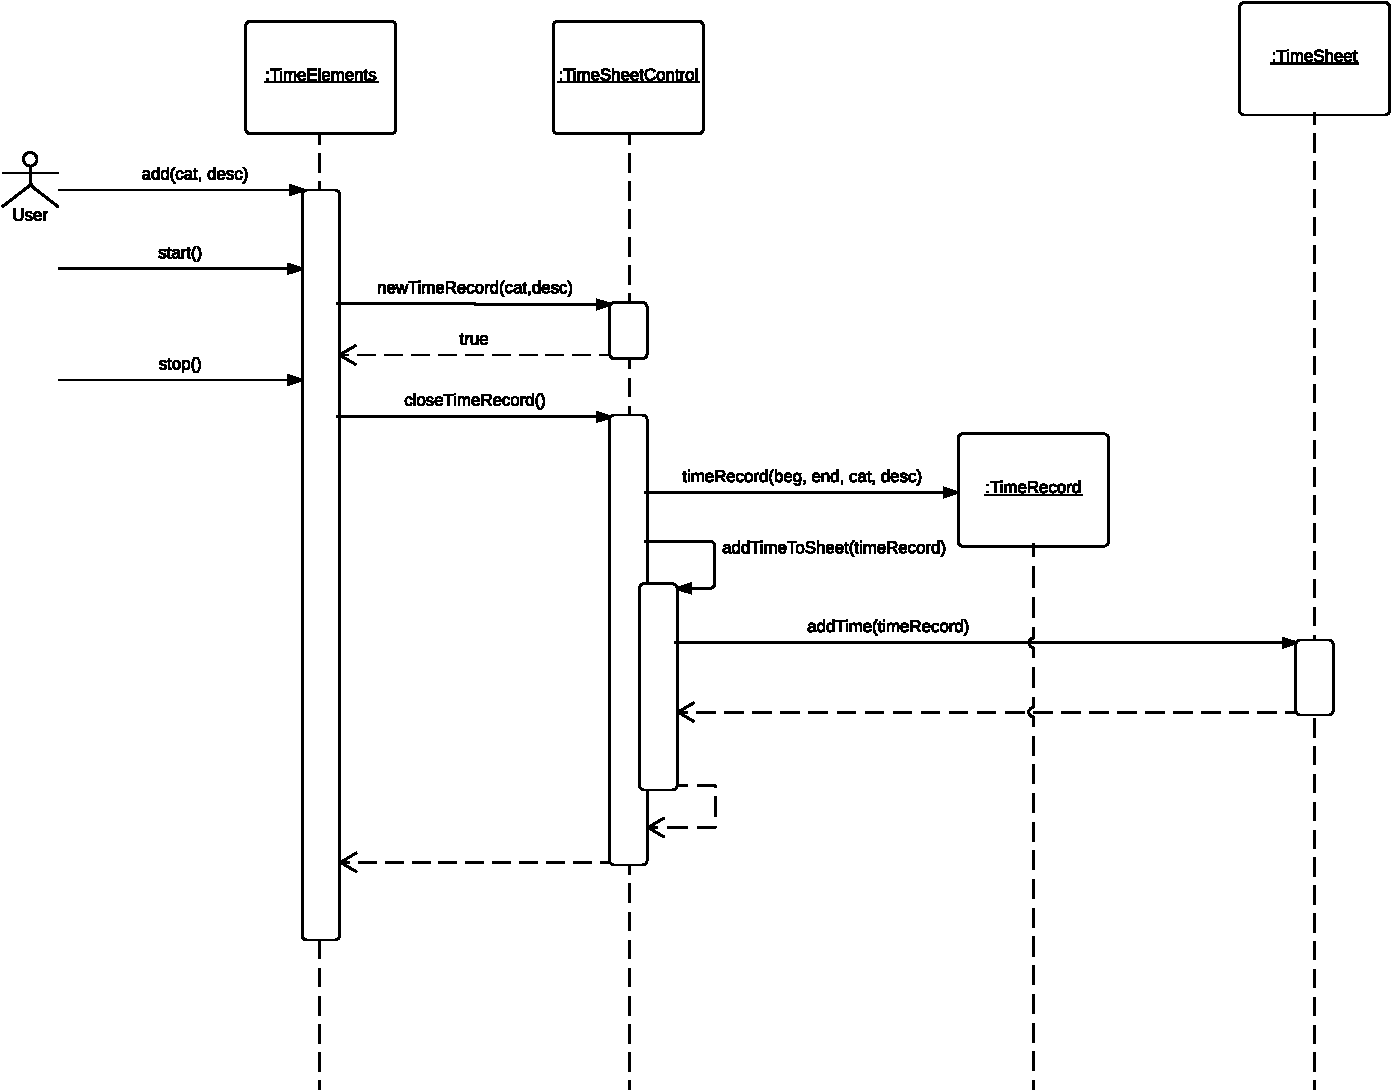
\includegraphics[width=\linewidth]{Diagramms/sequenzes/new_Time_record.pdf}

    \newpage
    \subsection{Login Sequenz}
        Ein User loggt sich ein.
        Falls als Authentifizierung LDAP statt Local ausgewählt ist, wird die Anfrage von LoginView stattdessen an den LDAP-Server weitergeleitet.
        Nur nicht eingeloggte User können diese Aktion durchführen.
        Für diese ist dies die einzige erlaubte Aktion.\\

        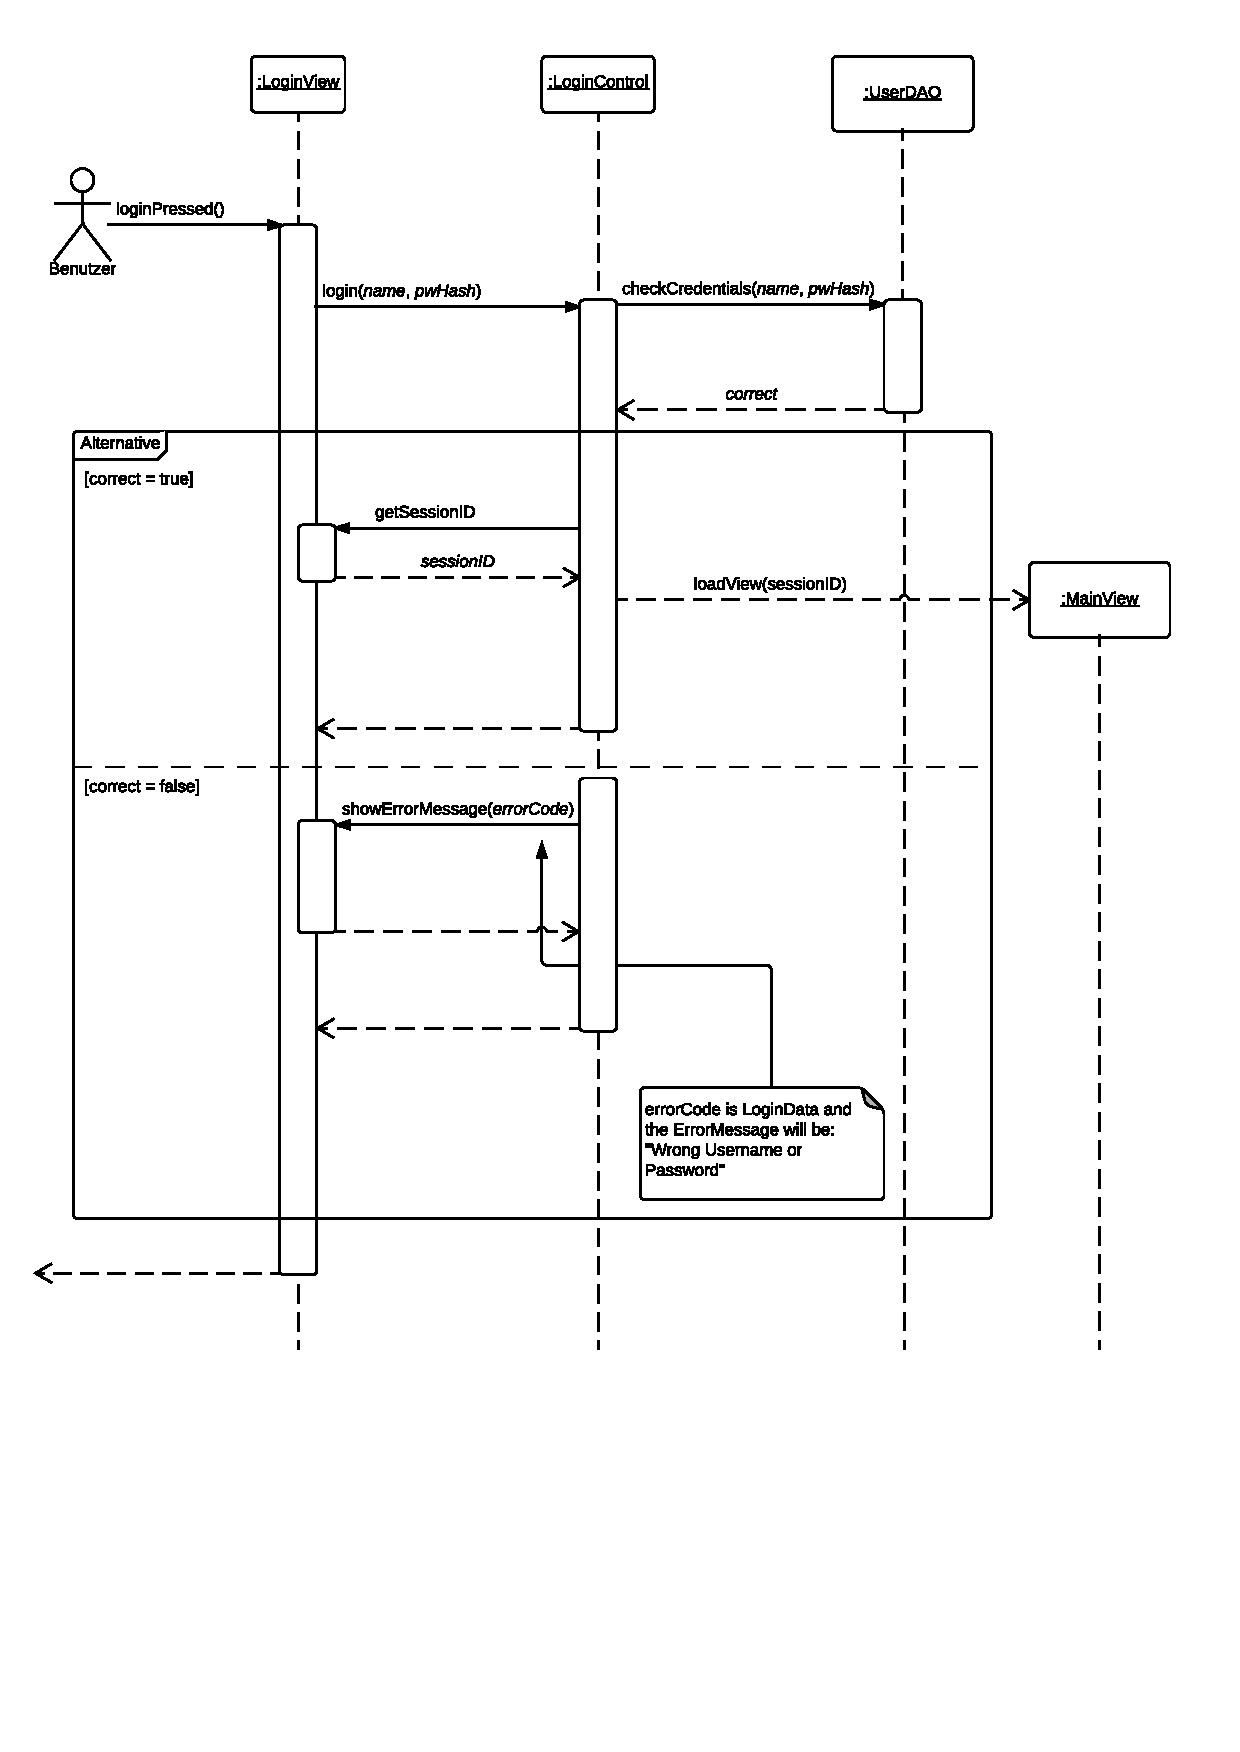
\includegraphics[width=\linewidth]{Diagramms/sequenzes/login.pdf}

    \newpage
    \subsection{Alle Stundenzettel der Gruppenmitglieder einsehen}
        Ein Supervisor lässt sich die Stundenzettel eines beliebigen Monats von allen von ihm betreuten Proletariern anzeigen.
        Supervisor können sich die Stundenzettel eines Monats von allen oder alle Stundenzettel eines von ihnen betreuten Proletariers anzeigen lassen.
        Administratoren können sich die Stundenzettel eines Monats aller Proletarier, nur aller von einem Supervisor betreuten Proletarier oder alle Stundenzettel eines Proletariers anzeigen lassen.
        Proletarier können diese Aktion nicht durchführen.\\

        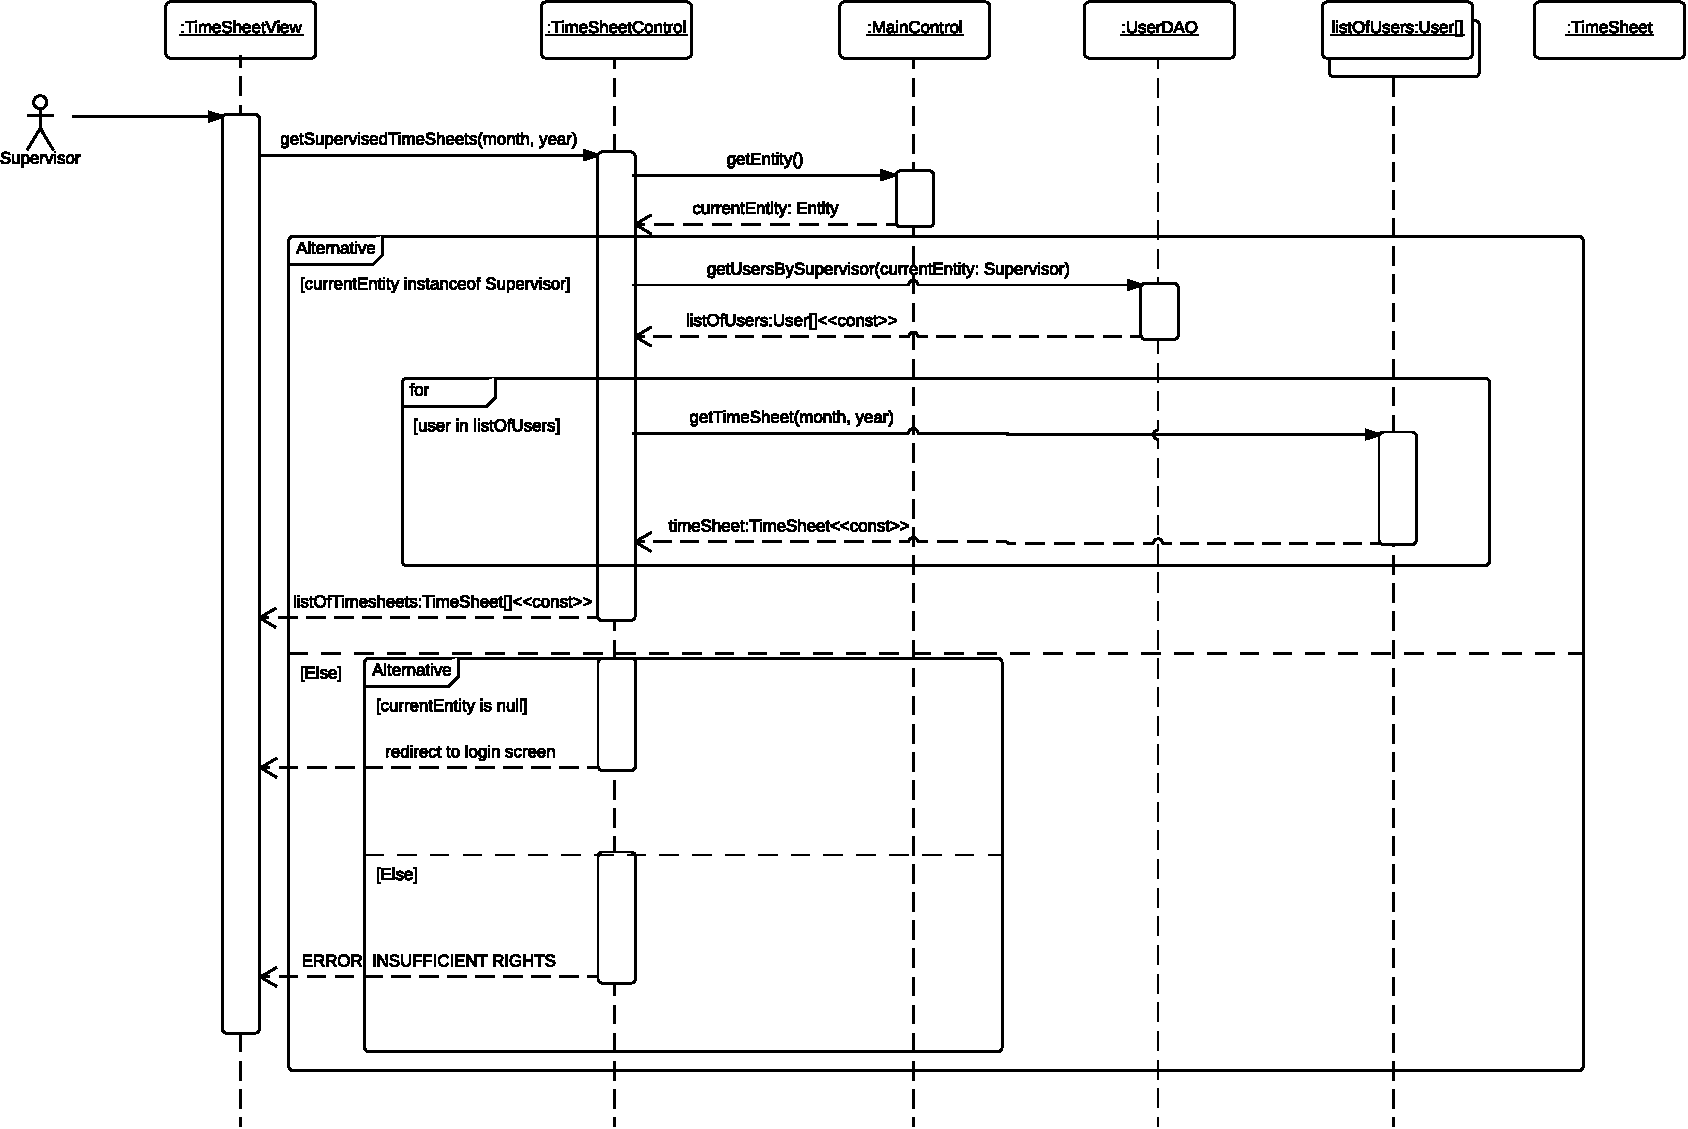
\includegraphics[width=\linewidth]{Diagramms/sequenzes/timesheets_of_all_supervised.pdf}

    \newpage
    \subsection{Aktuellen Stundenzettel einsehen}
        Ein Supervisor lässt sich den eigenen Stundenzettel des aktuellen Monats und die dazugehörigen Zeiterfassungen anzeigen.
        Diese Aktion kann für einen beliebigen Monat durchgeführt werden, solange ein Stundenzettel dafür existiert.
        Diese Aktion kann von Proletariern und Supervisorn durchgeführt werden.\\

        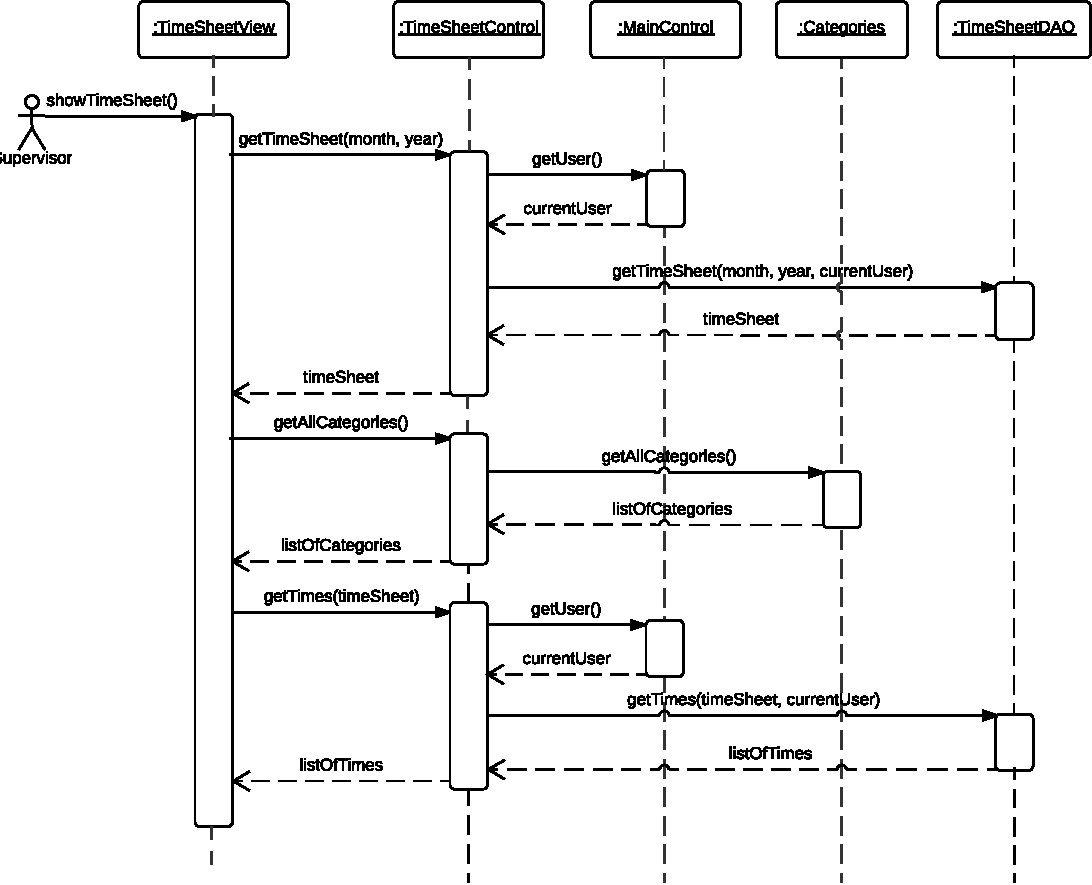
\includegraphics[width=\linewidth]{Diagramms/sequenzes/current_timesheet.pdf}

    \newpage
    \subsection{Stundenzettel abgeben}
        Ein Proletarier gibt seinen fertigen Stundenzettel ab.
        Dabei wird der Stundenzettel auf Fehler oder ähnliches überprüft und dann auf locked gesetzt.
        Dabei wird der Betreuer per Nachricht darüber informiert, damit dieser den Stundenzettel überprüfen kann.
        Diese Aktion kann von Proletariern und Supervisern ausgeführt werden.
        Superviser können außerdem Stundenzettel der von ihnen betreuten Proletarier von locked auf unlocked bzw. checked setzen.\\

        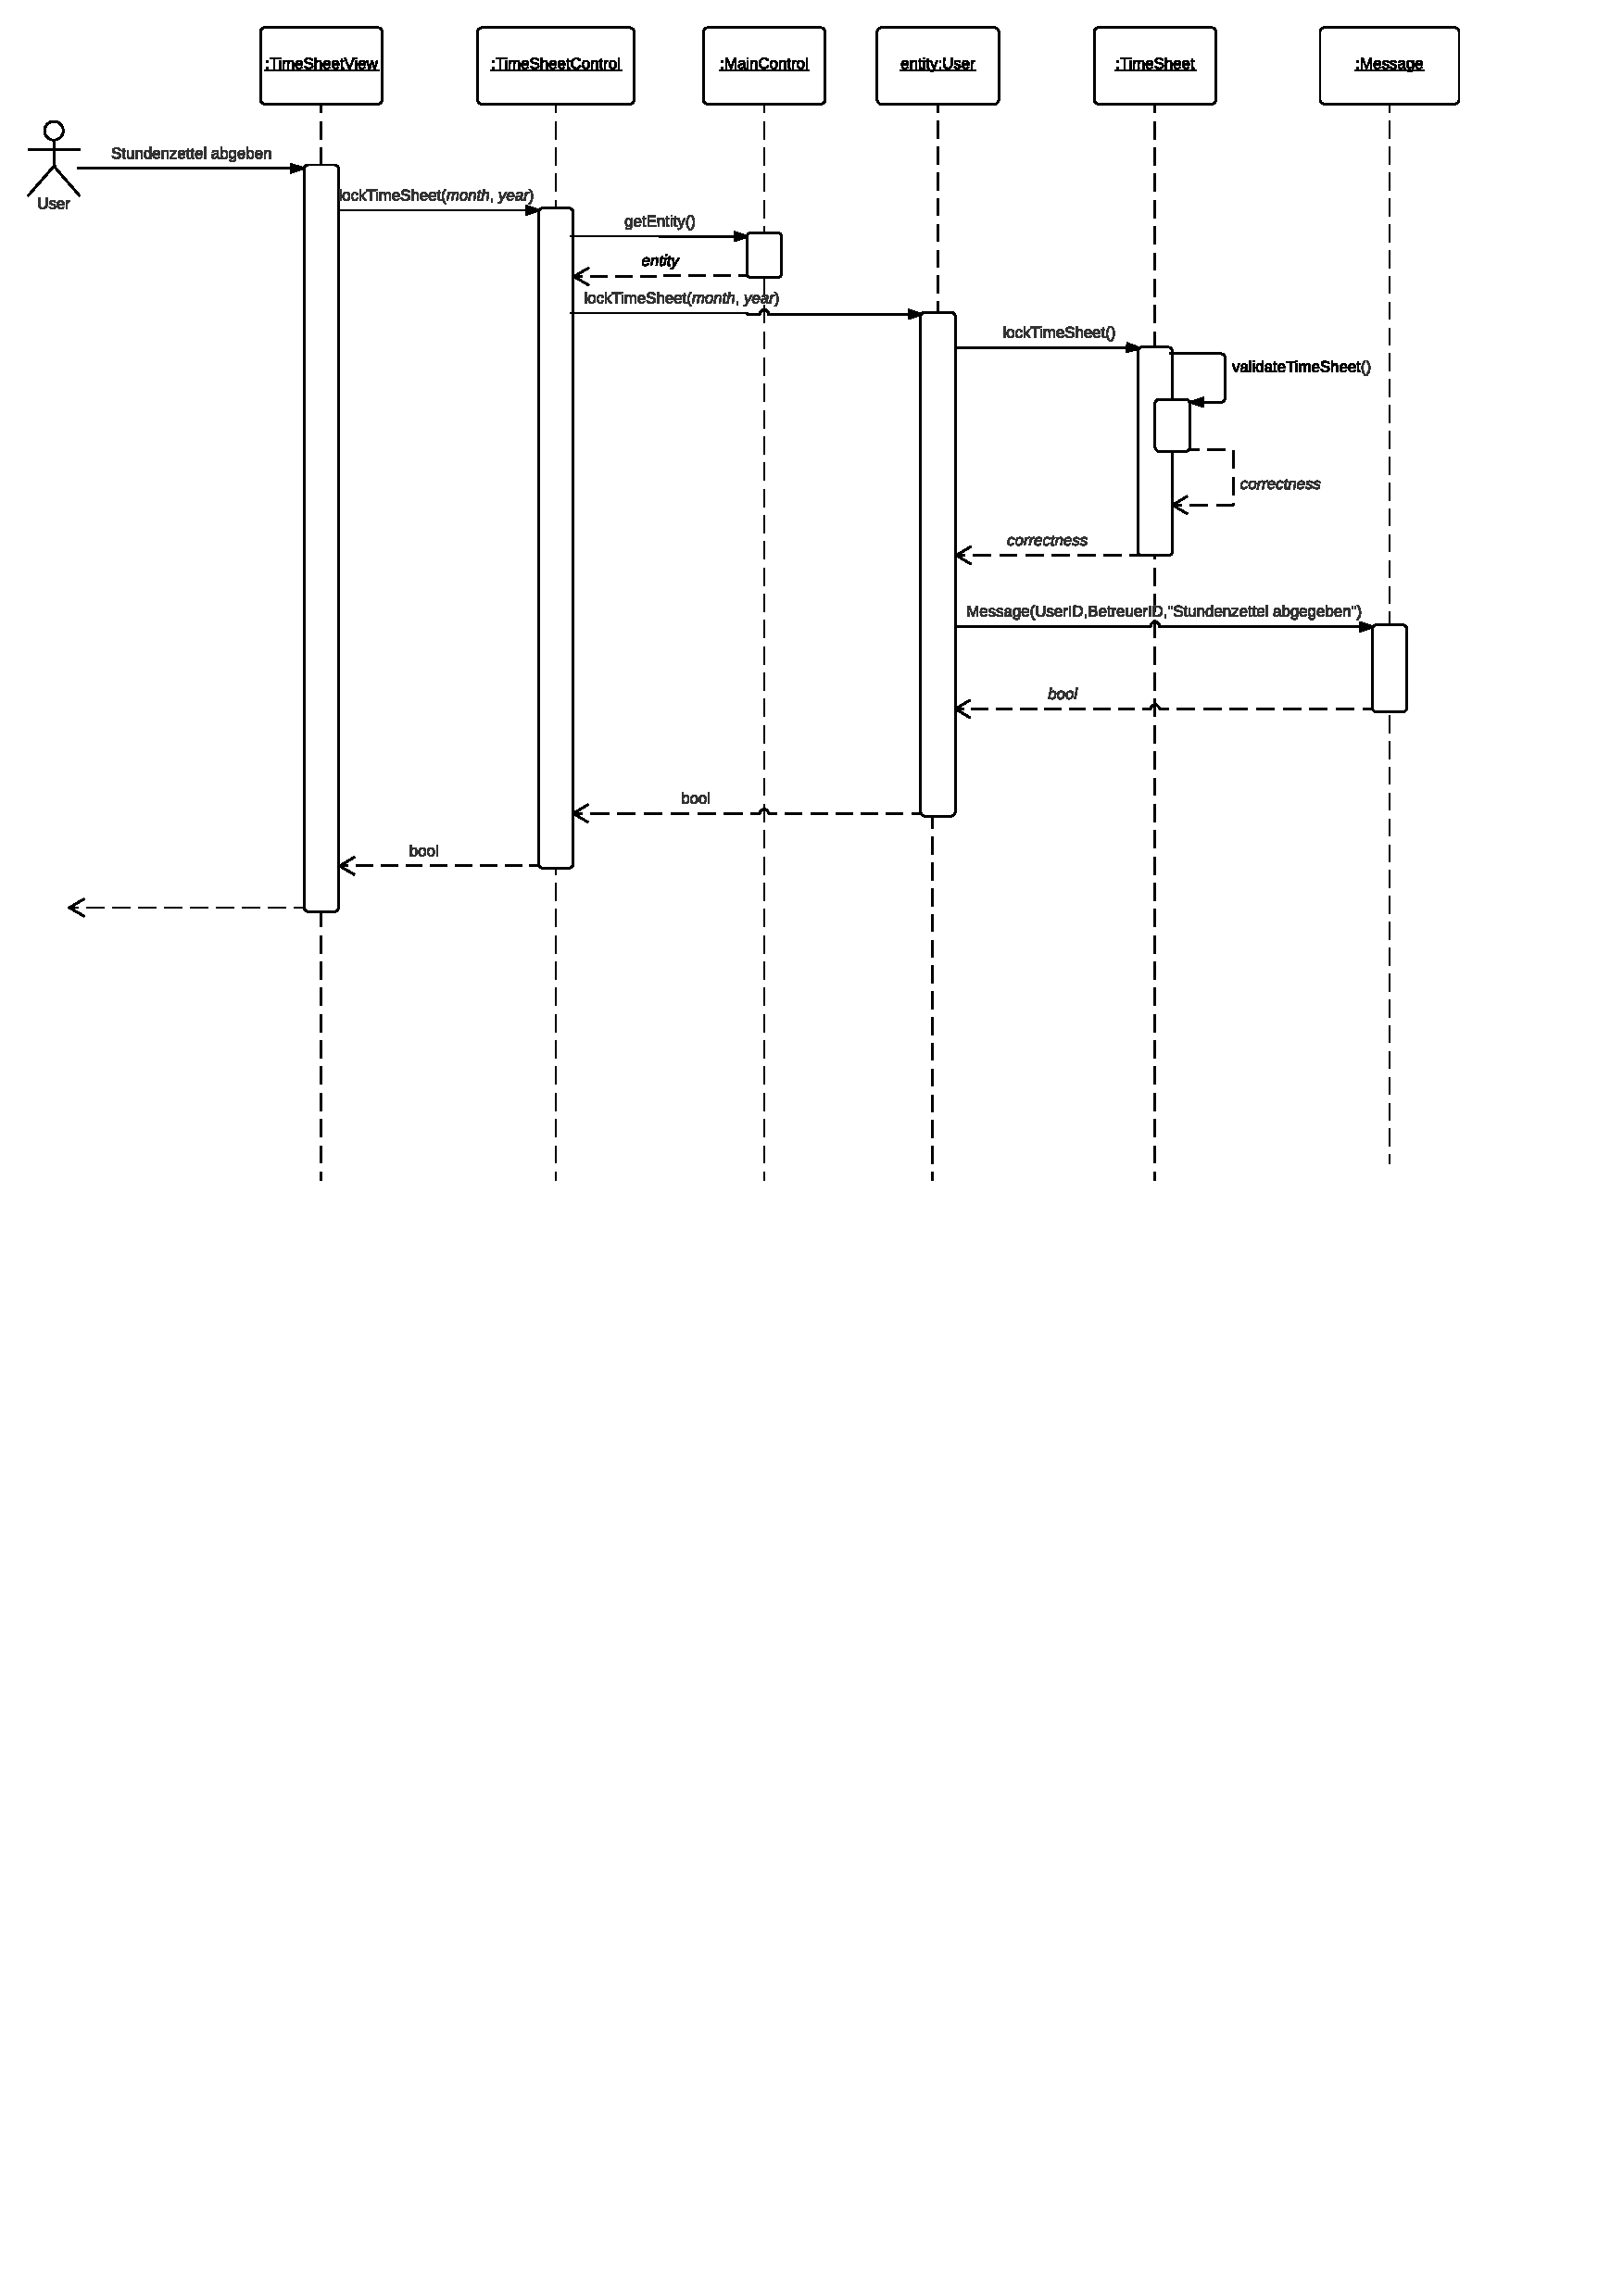
\includegraphics[width=\linewidth]{Diagramms/sequenzes/send_in_timesheet.pdf}

    \newpage
    \subsection{Benutzer anlegen}
        Ein neuer User wird angelegt.
        Falls LDAP zur Authentifizierung genutzt wird, muss kein Passwort angegeben werden.
        Falls ein Administrator angelegt wird, muss name, supervisor und hoursPerMonth nicht angegeben werden.
        Falls ein Supervisor angelegt wird, muss supervisor nicht angegeben werden.
        Diese Aktion kann nur von Administratoren ausgeführt werden.\\

        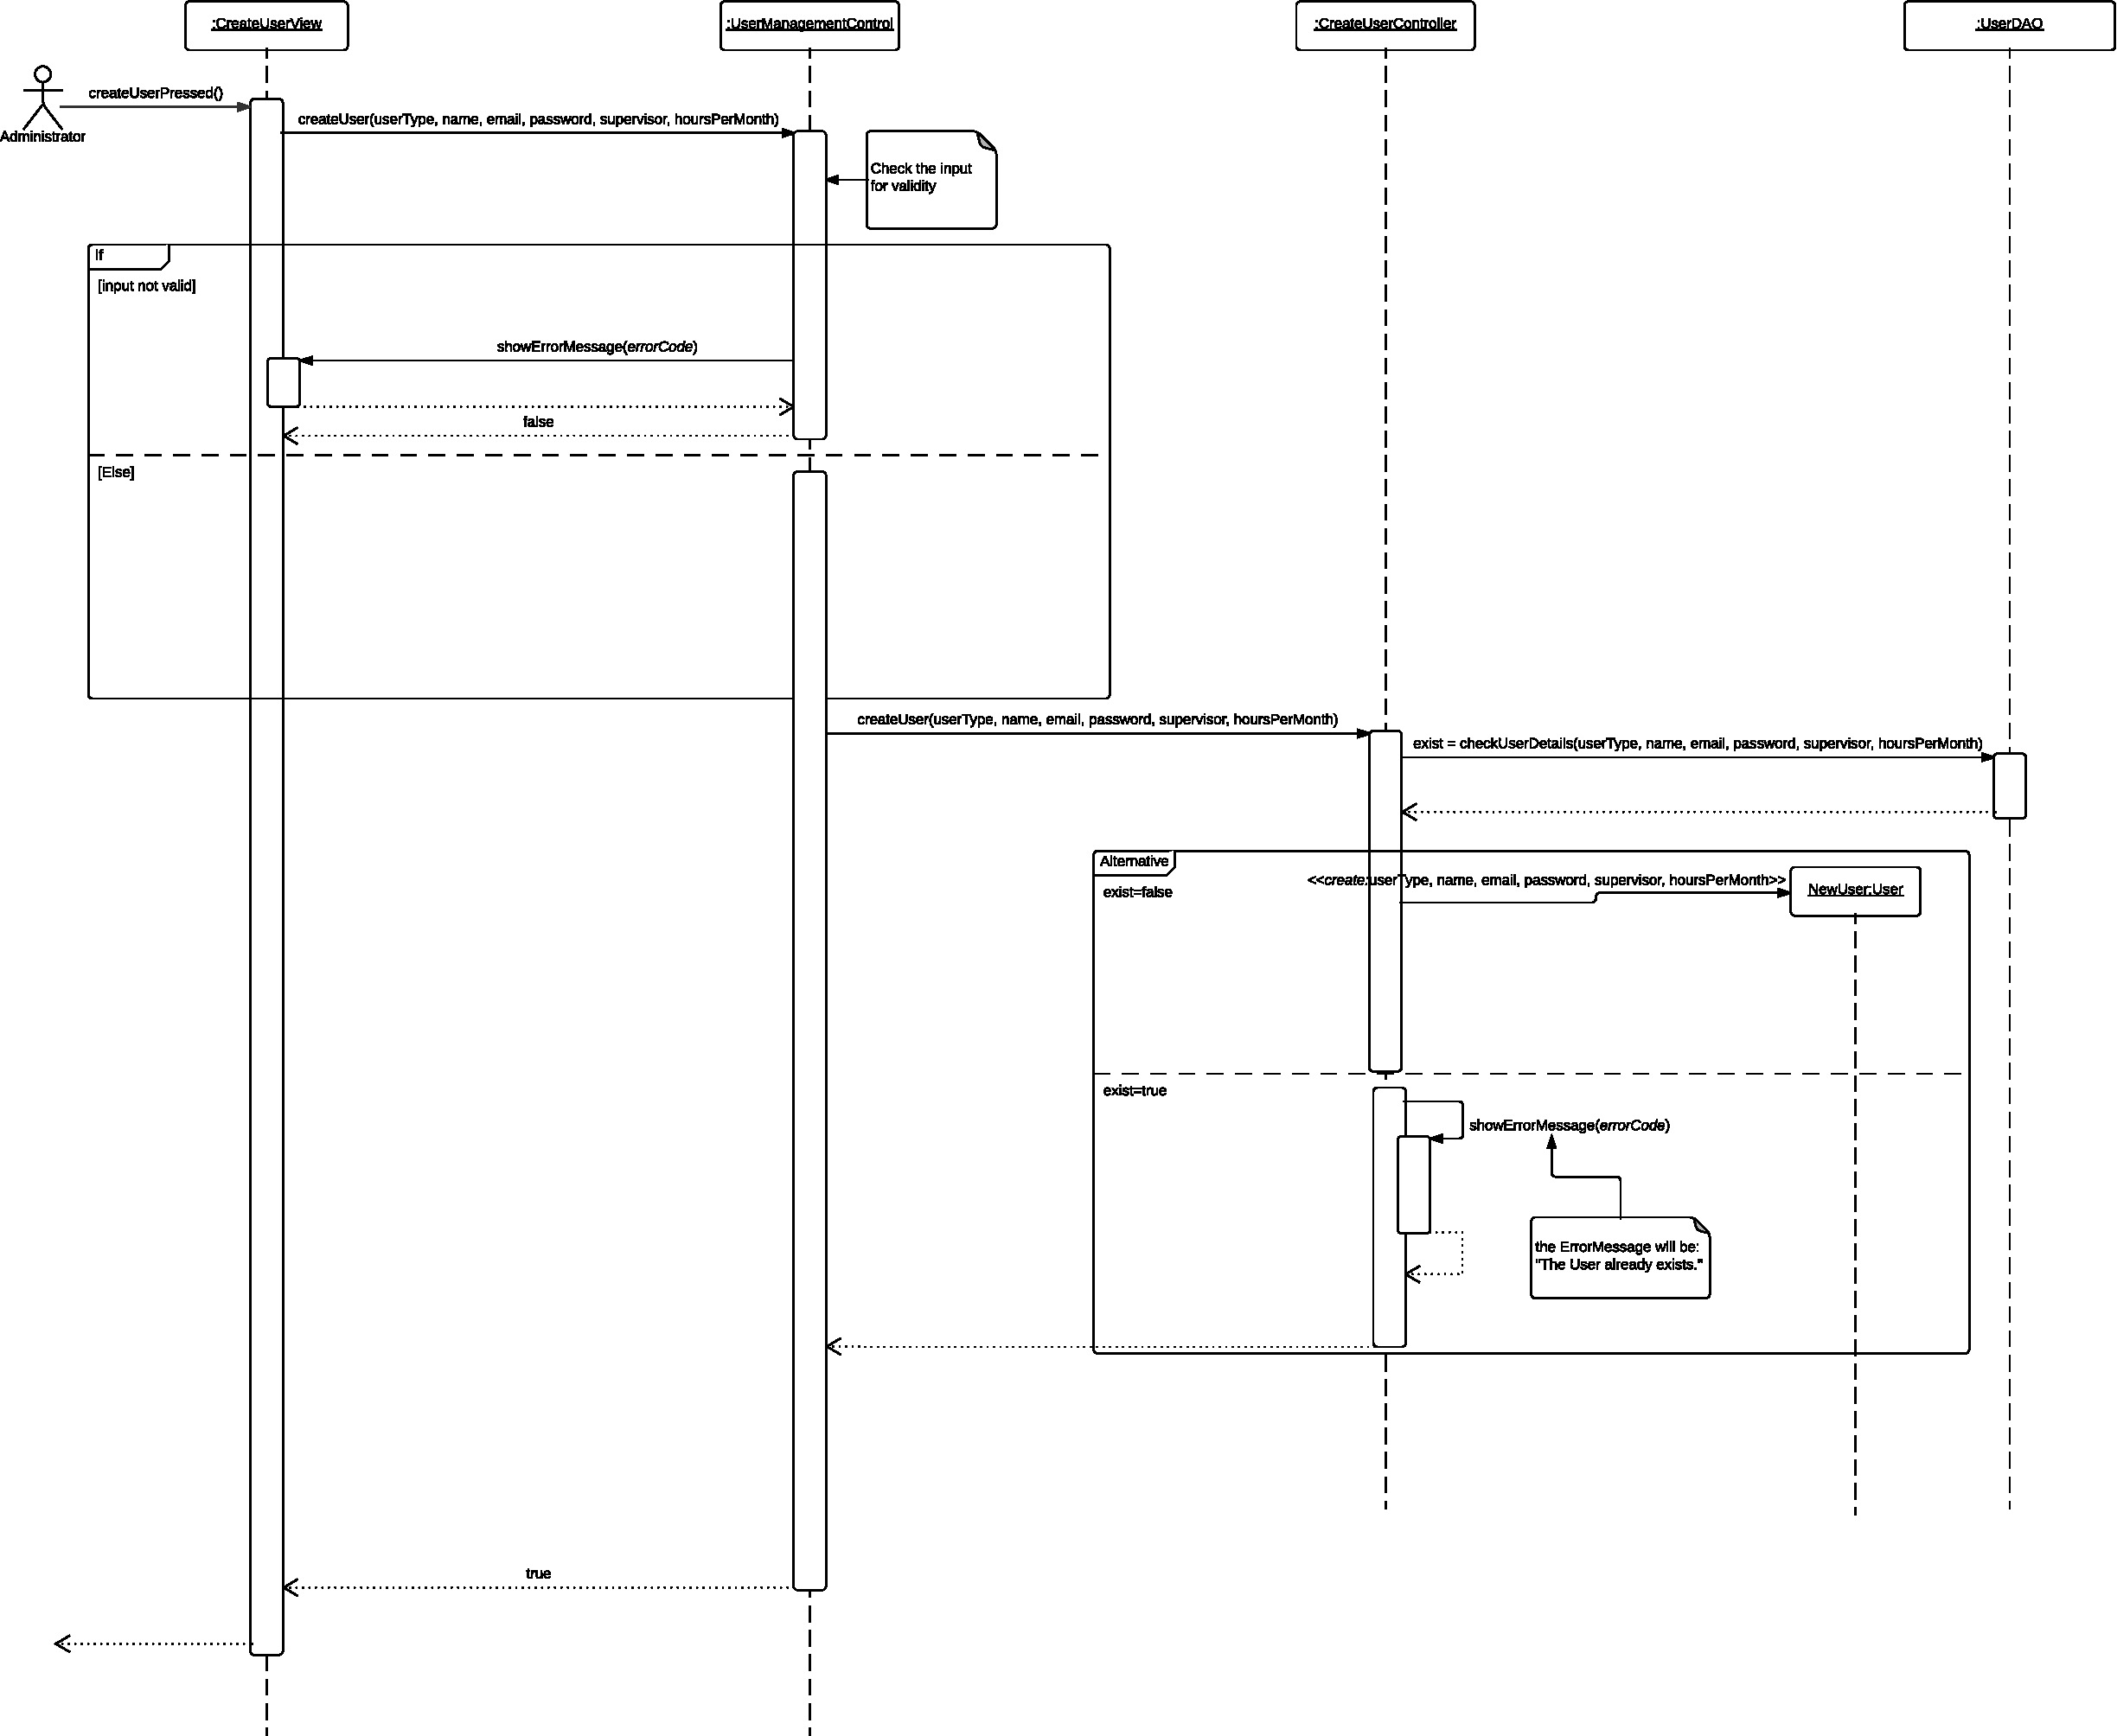
\includegraphics[width=\linewidth]{Diagramms/sequenzes/create_user.pdf}

    \newpage
    \subsection{Nachrichten verschicken}
        Eine Nachricht wird von einem User an einen anderen User verschickt.\\

        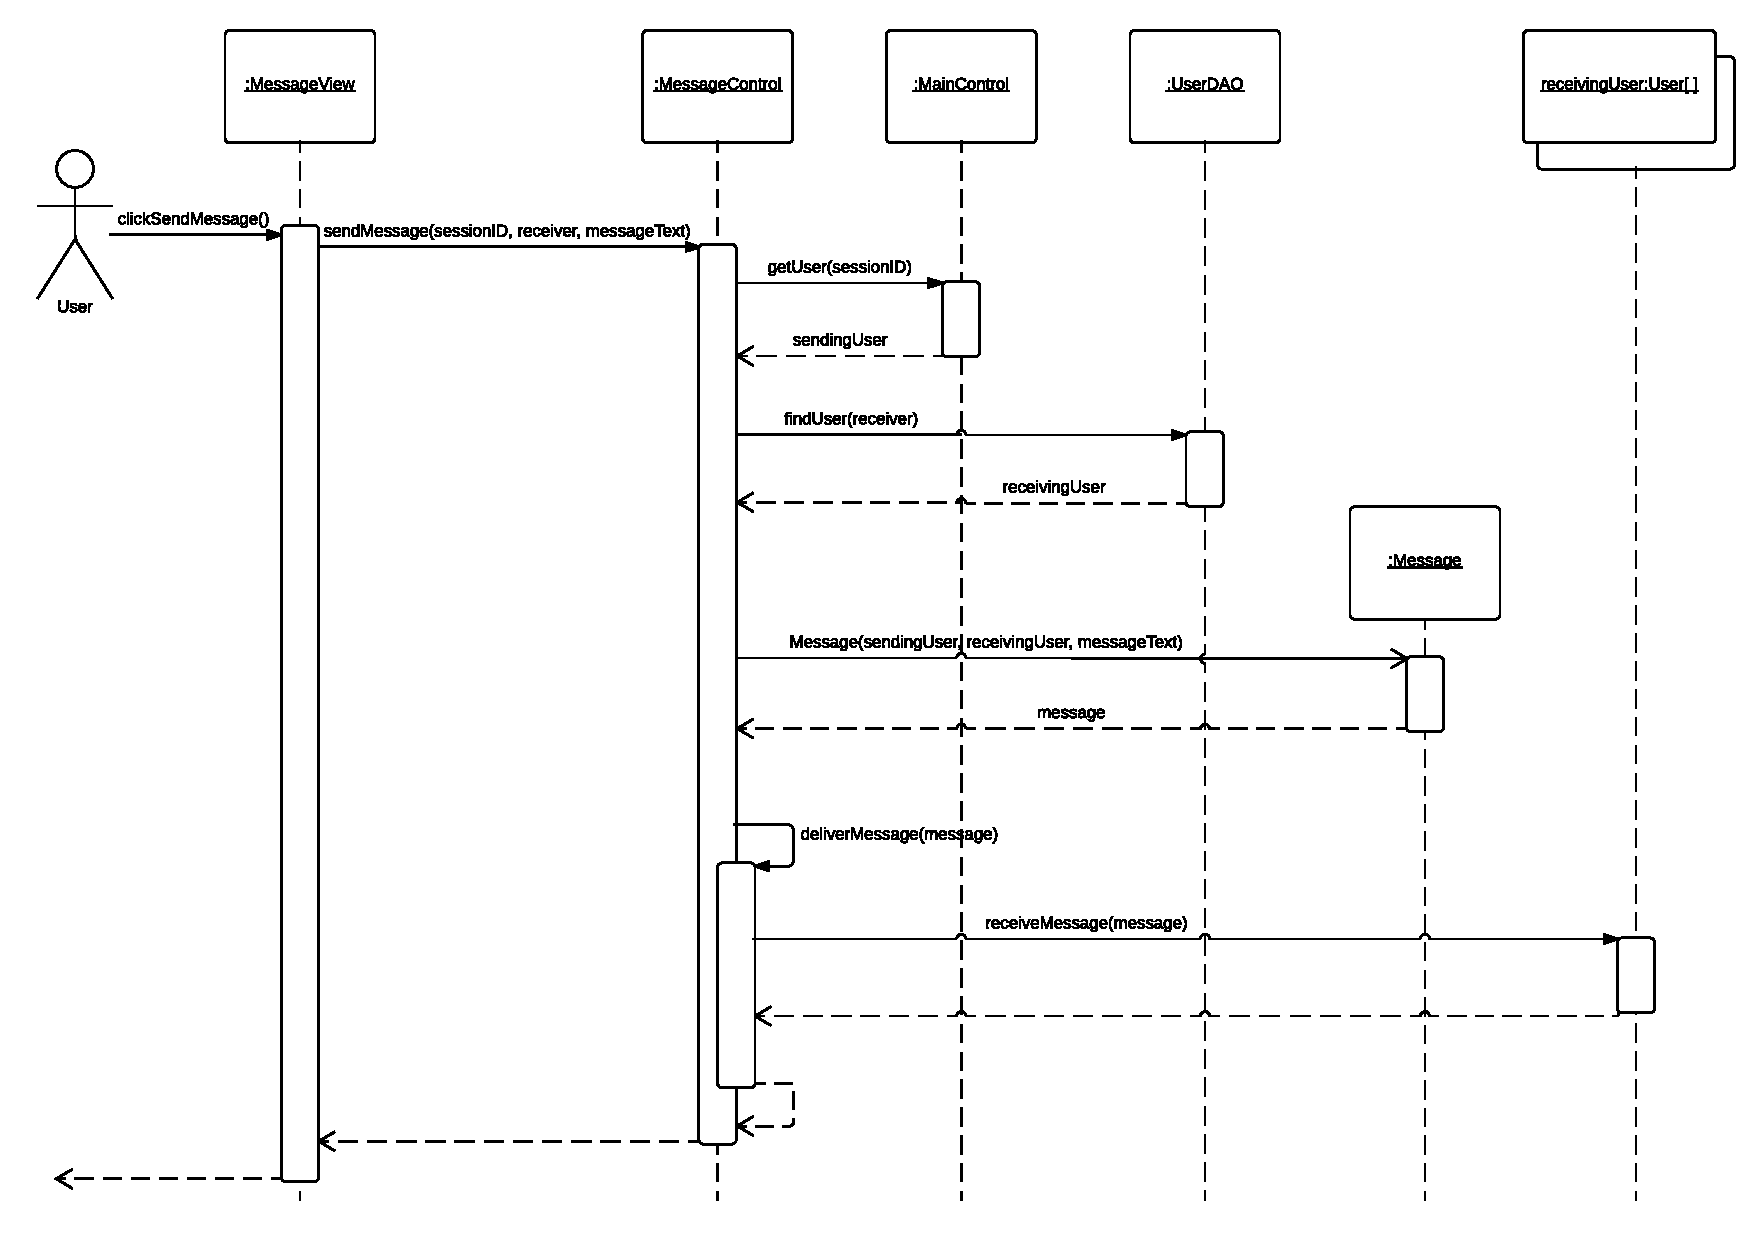
\includegraphics[width=\linewidth]{Diagramms/sequenzes/message_delivery.pdf}

    \newpage
    \subsection{Administrator exportiert alle Stundenzettel}
        Ein Administrator exportiert alle Stundenzettel eines Monats als ein zusammenhängendes pdf die den Status checked haben.
        Administratoren können zudem alle Stundenzettel eines Monats unabhängig vom Status, einen oder alle Stundenzettel eines Proletariers exportieren.
        Proletarier können einen oder alle ihre Stundenzettel exportieren.
        Supervisor können von ihren betreuten Proletariern alle Stundenzettel eines Monats die checked sind oder unabhängig von ihrem status exportieren.
        Zudem können sie einen oder alle Stundenzettel eines von ihnen betreuten Proletariers exportieren.\\

        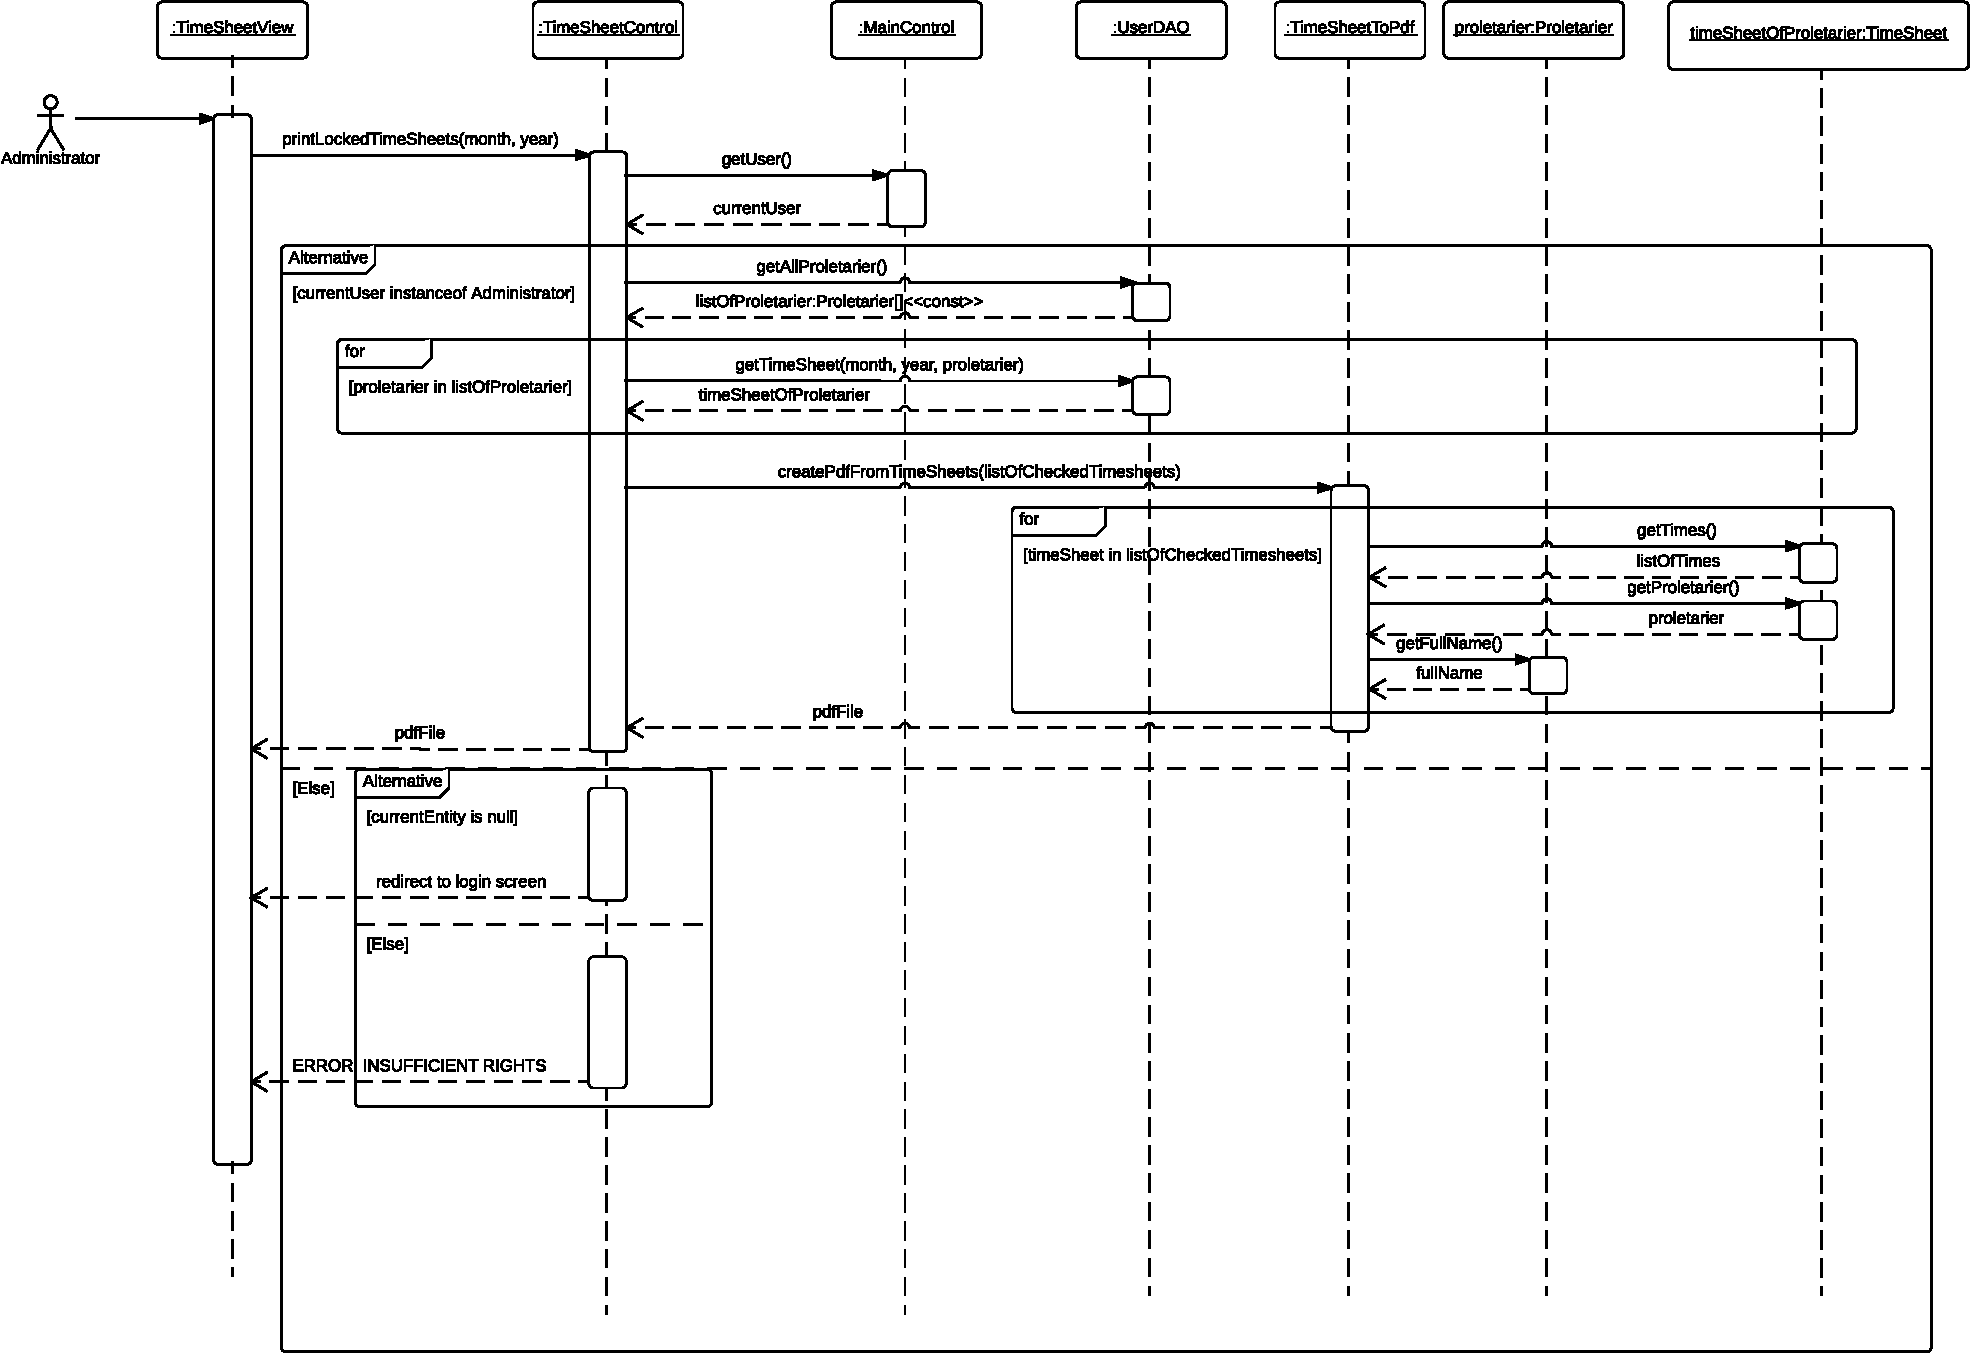
\includegraphics[width=\linewidth]{Diagramms/sequenzes/admin_prints_timesheets.pdf}

    \newpage
    \subsection{Alle Stundenzettel mit Zustand unlocked prüfen}
        Alle Stundenzettel mit dem Zustand unlocked werden auf inkonsistenzen geprüft, zum Beispiel ob der Proletarier gewarnt werden muss, dass der Stundenzettel abgegeben werden muss.\\

        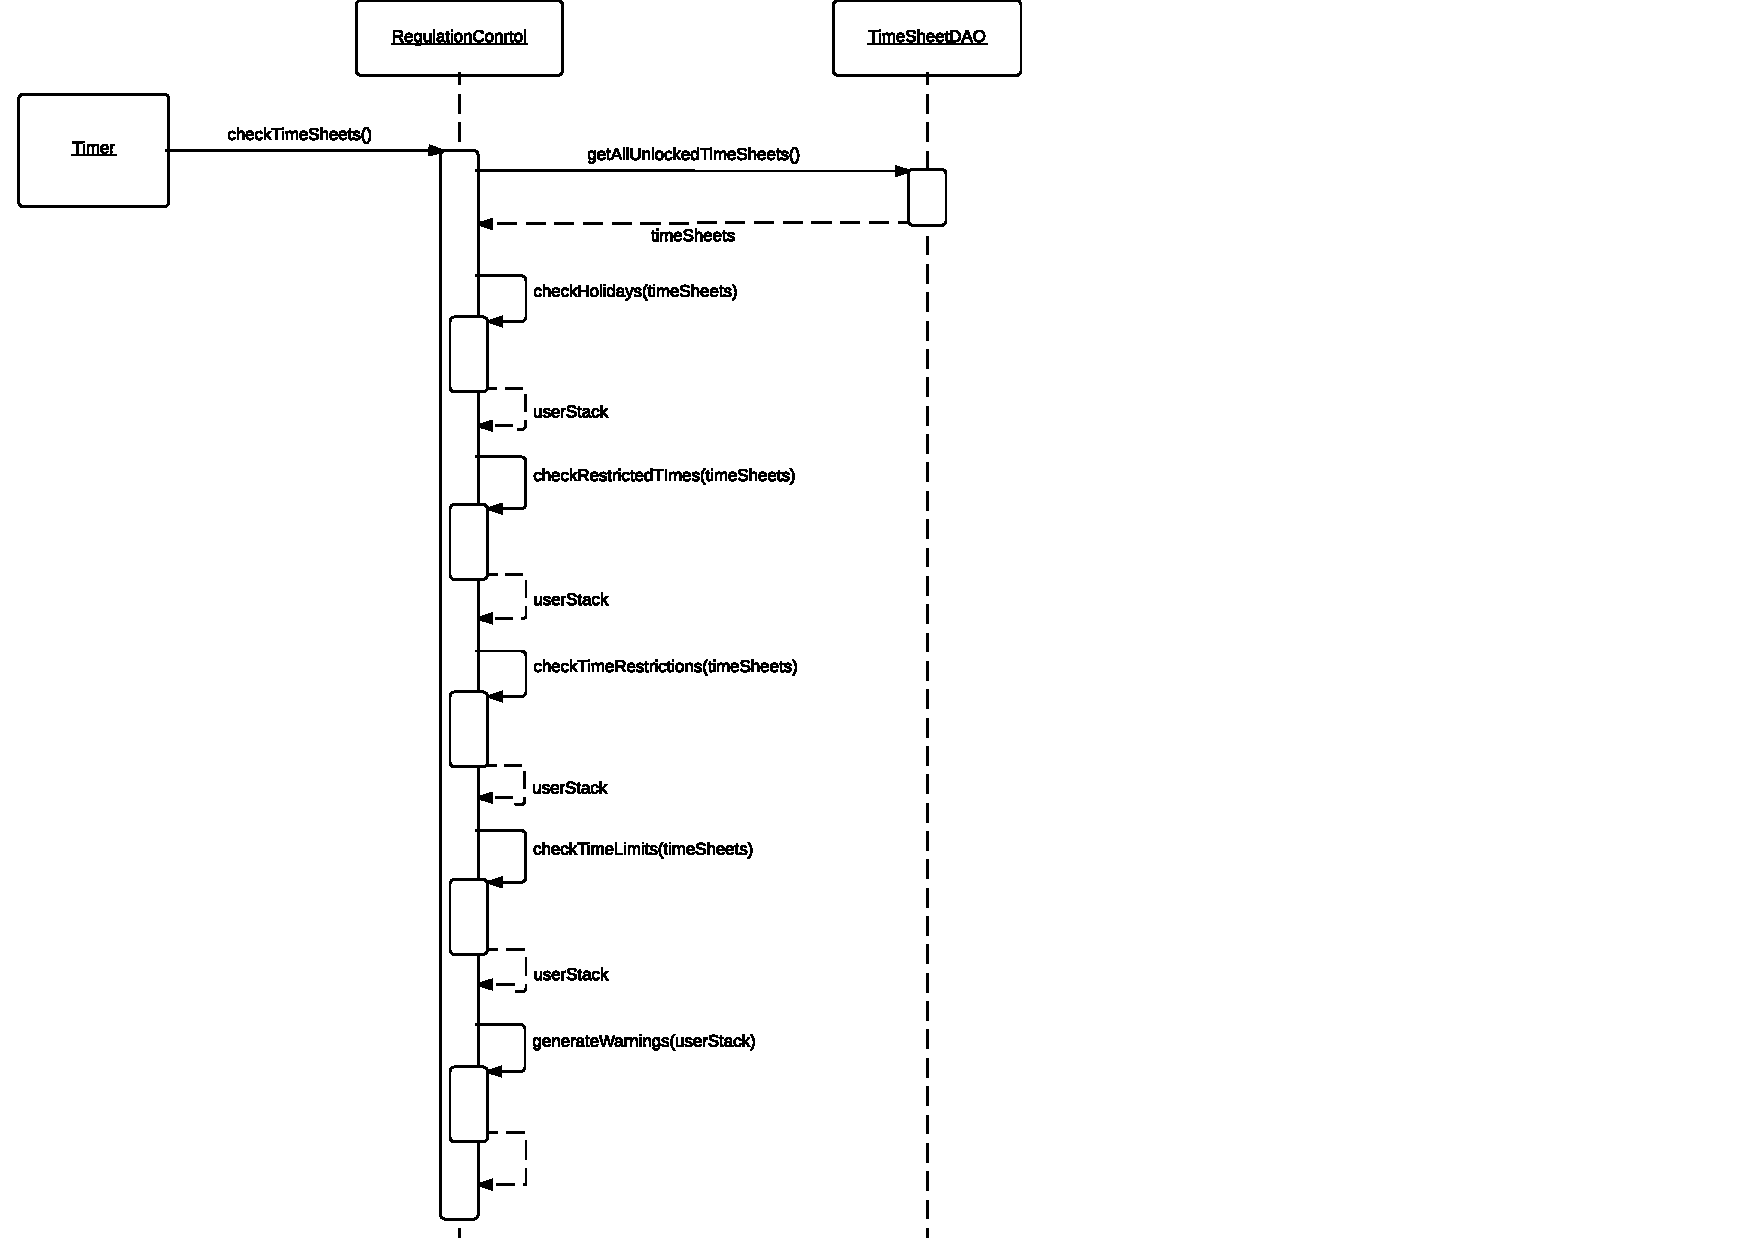
\includegraphics[width=\linewidth]{Diagramms/sequenzes/check_inconsistencies.pdf}

    \newpage
    \subsection{Prüfung eines Stundenzettels auf Rechtskonformität}
        Ein Stundenzettel wird auf Rechtskonformität geprüft.
        Dies beinhaltet die folgenden gesetzlichen Regelungen:
        \begin{itemize}
            \item Die gesetzlich maximale Arbeitszeit wird nicht überschritten (§3 ArbZG).
            \item Die gesetzliche Pausenzeiten werden eingehalten (§4 ArbZG).
            \item Die Ruhezeiten wurden eingehalten (§5 ArbZG).
            \item Es hat keine Nachtarbeit stattgefunden (§6 ArbZG).
            \item Die Sonn- und Feiertagsruhe wurde eingehalten (§9 ArbZG).
                Dabei werden nur die Feiertage in Baden-Württemberg beachtet.
        \end{itemize}

        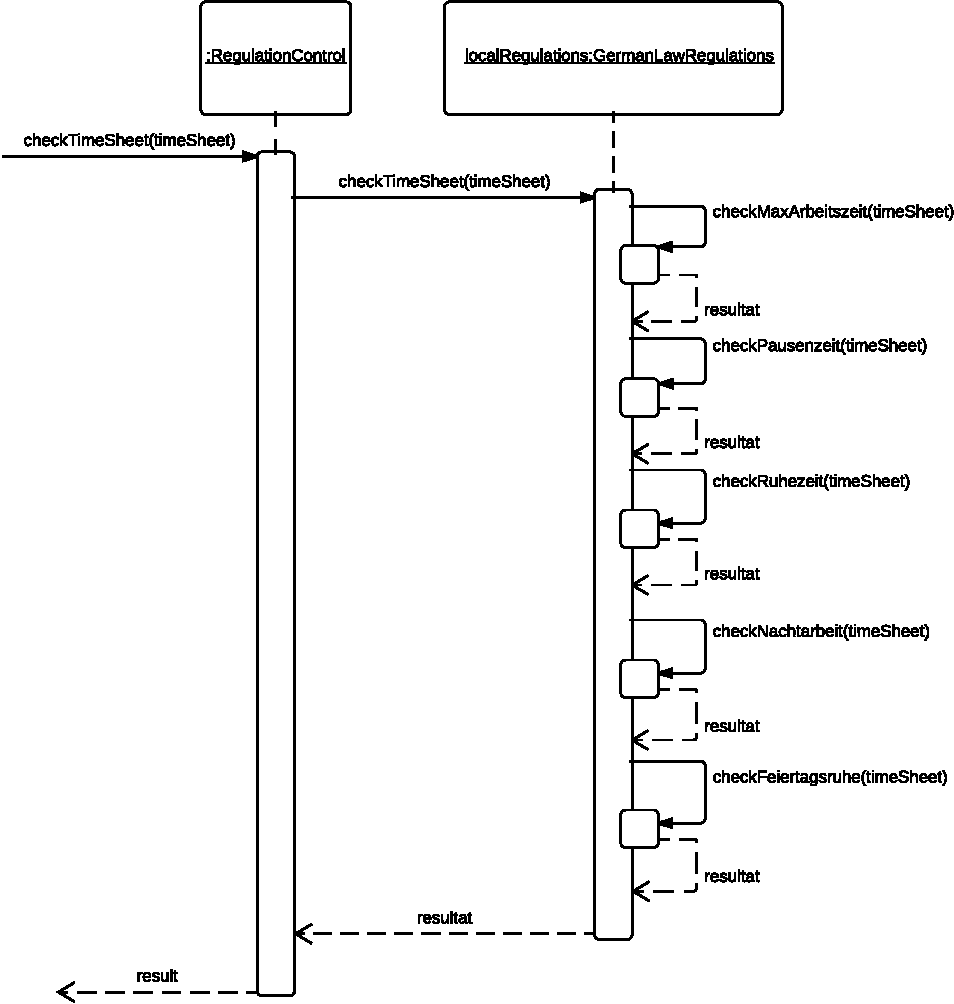
\includegraphics[width=\linewidth-2cm]{Diagramms/sequenzes/check_german_law_regulations.pdf}

	\section{Datenbankdesign}

\subsection{ER Diagramm}
    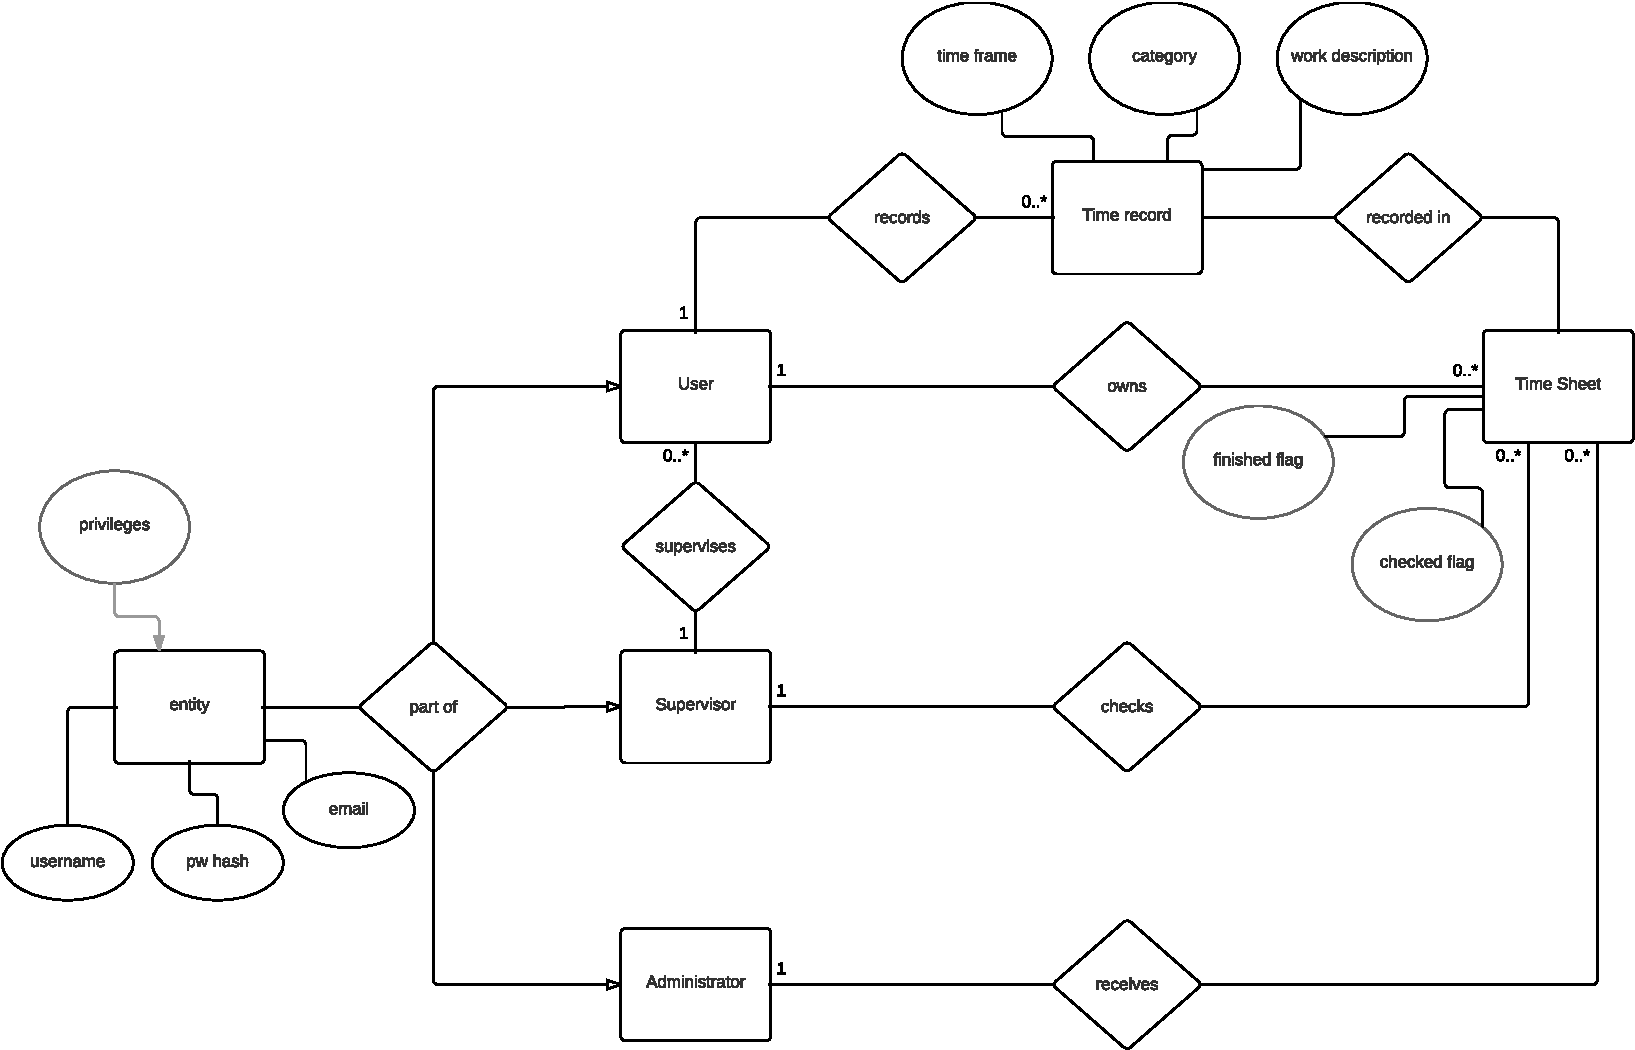
\includegraphics[width=\linewidth]{Diagramms/erDiagramm}\\
\subsection{TODO name für dieses ding}
    \begin{itemize}
        \item Entity\{username(PK),pwHash,email, privilges\}
        \item timeSheet\{id(PK),username(FK), finishedFlag,checkedFlag\}
        \item Time\{id(PK), timeSheetID(FK), timeFrame, category, workDescription\}
    \end{itemize}

	\section{Dateiformate}
\subsection{Dateiformat zur Definition von gesetzlichen Feiertagen}
In einer Datei "`Feiertage.dat"' können die gesetzlichen Feiertage des entsprechenden Bundeslandes konfiguriert werden.
Ausgeliefert wird das Programm mit den gesetzlichen Feiertagen für Baden-Württemberg.
Wenn die Datei geändert wurde, muss das Programm danach neu kompiliert werden, da im Quellcode eine Prüfsumme der Datei hinterlegt ist um Manipulation zu erschweren.
Die Datei ist ASCII-kodiert.

In jeder Zeile steht der Name eines Feiertags gefolgt von einem Doppelpunkt und dem Datum.
Das Datum kann auf zwei Arten hinterlegt werden:
\begin{itemize}
    \item Das Datum im Format TT.MM., also zum Beispiel 05.01.
    \item Als Anzahl der Tage vor oder nach dem Osterdatum, im Format +N bzw -N, also zum Beispiel +60
\end{itemize}

\subsection{Datenbankanbindung}
In der Datei "`hibernate.cfg.xml"' wird die Datenbankanbindung mittels der Variablen connection.driver\_class, connection.url, connection.username und connection.password definiert.
Diese Datei muss
Die Syntax der Datei entspricht den Vorgaben von Hibernate ORM 5.0.

\subsection{Authentifizierung via LDAP}
Falls die Authentifizierung via LDAP erwünscht ist, muss die Anbindung der "`Shiro.ini"' konfiguriert werden.
Die Syntax der Datei entspricht den Vorgaben von Shiro 1.2.4.

	\section{Glossar}
\begin{description}
	\item[Administrator*] Der \emph{Administrator*}. Höchste Entität, besitzt Rechte zum modizieren von angelegten \emph{Benutzern*}.
	               Erhält ebenfalls die \emph{abgegebenen Stundenzettel}.

	\item[ArbZG] Das deutsche Arbeitszeitgesetz

	\item[Betreuer*] Betreut mehrere \emph{Benutzer*} und kann deren \emph{Stundenzettel} einsehen.

	\item[Heatmap] Eine \emph{Heatmap} ist ein Diagramm zur Visualisierung von Daten, deren abhängige Werte einer zweidimensionalen Definitionsmenge als Farben repräsentiert werden.  \emph{(Zitat Wikipedia)}

	\item[JDBC] Eine Bibliothek um eine Vielzahl an Datenbanken nutzen zu können (z.B. MySQL oder PostgreSQL)

	\item[Kategorie] In welche \emph{Kategorie} die \emph{Tätigkeit} fällt. Zum Beispiel an welchem Projekt gearbeitet wurde

	\item[Session cookie] Eine Information die im Browser des \emph{Benutzers*} hinterlegt wird um ihn zu identifizieren, damit er nicht bei jeder Aktion sein Passwort neu eingeben muss.

	\item[Stundenzettel] Formular auf dem die geleisteten Stunden mit \emph{Tätigkeit} vermerkt werden.

	\item[Team] Gruppe von \emph{Benutzern*} die von einem \emph{Betreuer*} geleitet werden.

	\item[*] Der * bei \emph{Benutzer*} (und auch \emph{Betreuer*} und \emph{Administrator*}) deutet an, dass die Rolle von Personen jeden Geschlechts eingenommen werden kann, nicht nur von Personen die sich mit er/sein (oder sie/ihr) Pronomen identifizieren.

\end{description}



\end{document}
